
\documentclass[11pt]{article}

\usepackage{xcolor}
\usepackage{mathtools}
\usepackage[legalpaper, margin=1in]{geometry}
\usepackage{amsmath}
\usepackage{amssymb}
\usepackage{paralist}
\usepackage{rsfso}
\usepackage{amsthm}
\usepackage[inline]{enumitem}   

\newtheoremstyle{break}
  {\topsep}{\topsep}%
  {\itshape}{}%
  {\bfseries}{}%
  {\newline}{}%
\theoremstyle{break}
\theoremstyle{break}
\newtheorem{axiom}{Axiom}
\newtheorem{thm}{Theorem}[section]
\newtheorem{lem}{Lemma}[thm]
\newtheorem{prop}[lem]{Proposition}
\newtheorem{corL}{Corollary}[lem]
\newtheorem{corT}[lem]{Corollary}
\newtheorem{defn}{Definition}[corL]

\newcommand{\R}{\mathbb{R}}
\newcommand{\N}{\mathbb{N}}
\newcommand{\Z}{\mathbb{Z}}
\newcommand{\Q}{\mathbb{Q}}
\newcommand{\A}{\mathcal{A}}
\newcommand{\J}{\mathcal{J}}
\newcommand{\T}{\mathcal{T}}
\newcommand{\C}{\mathcal{C}}
\newcommand{\M}{\mathcal{M}}
\newcommand{\Complex}{\mathbb{C}}
\newcommand{\Power}{\mathcal{P}}
\newcommand{\pd}{\partial}
\newcommand{\ee}[1]{\cdot 10^{#1}}
\newcommand{\lr}[1]{\left( #1 \right)}
\newcommand{\ihat}{\hat{\i}}
\newcommand{\jhat}{\hat{\j}}
\newcommand{\khat}{\hat{k}}
\newcommand{\dbar}{d\hspace*{-0.08em}\bar{}\hspace*{0.1em}}

\newcommand{\note}{\color{red}Note: \color{black}}
\newcommand{\remark}{\color{blue}Remark: \color{black}}
\newcommand{\example}{\color{green}Example: \color{black}}
\newcommand{\exercise}{\color{green}Exercise: \color{black}}



\makeatletter
\def\@seccntformat#1{%
  \expandafter\ifx\csname c@#1\endcsname\c@section\else
  \csname the#1\endcsname\quad
  \fi}
\makeatother

\makeatletter
\newcommand*{\rom}[1]{\expandafter\@slowromancap\romannumeral #1@}
\makeatother

\makeatletter
% This command ignores the optional argument for itemize and enumerate lists
\newcommand{\inlineitem}[1][]{%
\ifnum\enit@type=\tw@
    {\descriptionlabel{#1}}
  \hspace{\labelsep}%
\else
  \ifnum\enit@type=\z@
       \refstepcounter{\@listctr}\fi
    \quad\@itemlabel\hspace{\labelsep}%
\fi}
\makeatother
\parindent=0pt


\begin{document}

	\begin{titlepage}
		\begin{center}
			\topskip0pt
			\vspace*{\fill}
			\Huge \color{red}
				\textbf{Class Notes}\\
			\vspace{0.5cm}			
			\Large \color{black}
				Physics 406 - Statistical Mechanics\\	
				University of Michigan\\
			\vspace{3cm}

			
			\vspace{5cm}
			\LARGE
				\textbf{Jinyan Miao}\\
				Winter 2022\\
			\vspace{5cm}

		\vspace*{\fill}
		\end{center}			
	\end{titlepage}

\newpage
\section{\color{red} Macroscopic and microscopic descriptions of physical systems}

For systems with large number of particles, we will try to find a microscopic description for such system, by assigning position $\vec{r}_i$ and momentum $\vec{p}_i$ for all the particles. If a system has $N$ particles, a \textbf{Phase Space} is the space of momenta and positions  of the particles, which has $3N$ position coordinates, $3N$ momenta coordinates, and hence a $6N$ dimensional space. The state of each particle in the system is a point in this phase space.

Macroscopic description of a system with large number of particles, with number of particles $\geq \ee{23}$, uses the macroscopic variables such as $V$, $N$, $T$, and so on. Thermodynamics describes the macroscopic relation between the macroscopic parameters of the system without any reference to microscopic properties.\\

Statistical mechanics is the microscopic description of the \\

Whenever you give a macroscopic description, there is () meaning about the microscopic state of the system. There can be many microstate that give the same macroscopic parameters.\\


Consider there spins in a magnetic field. Spin up has energy $-\mu H$, and spin down has energy $+\mu H$. \\
The following are some of the microstates:
\begin{enumerate}[topsep=3pt,itemsep=-1ex,partopsep=1ex,parsep=1ex]
\item (up) (up) (up)
\item (up) (up) (down)
\item (down) (up) (up)
\item (up) (down) (up)
\item (down) (down) (up)
\item etc.
\end{enumerate}
For cases (2), (3), and (4), all have total energy $-\mu H$, they are microstates consisting of two ups and one down. If one fixes the macroscopic state by specifying the total energy, say $E_{total} = -\mu H$, we observe that there are three microstates that give the same macroscopic description. To generalize, when one specifies a macrostate, there is information missing about the microstate of such system. Many microstates will give the same macrostate. The sates correspond with a given macrostate are called the accessible states. In this example, only three microstates are accessible to the total energy $E_T = -\mu H$. This is where probability comes in to the description and hence irreversible problem. 

\newpage
\section{\color{red} Notes on Probability Theory}
Let $P_r$ denotes a discrete probability, we have $1\geq P_r \geq 0$, with $\sum_r P_r = 1$.\\

When we have large number of systems, discrete probabilities become continuous values, and here we get a probability distribution, $P(x)\, dx$ is the probability that \\


For average values:\\
In discrete probability $P_r$, given $f(r)$, average is given by: $$\bar{f} = \sum_r f(r) P_r$$\\
In continuous probability $P(x)$, given $f(r)$, average is given by $$\bar{f} = \int_{-\infty}^\infty P(x) f(x)\, dx$$ \\

Binomial distribution plays a special role. Suppose one makes $N$ independent trials, the probability of a "hit" is $p$, and the probability of a "miss" is $q$, with $p+q = 1$. Then the probability of exactly $m$ "hits" in $N$ trials is given by the following:
$$P_m = \frac{N!}{m!(N-m)!}p^m q^{N-m}$$
and we have $\sum_m P_m = 1$.


For mean values of binomial distribution:
\begin{align*}
\bar m &= \sum_{m=0}^N mP_m = \sum_{m=0}^N \frac{N! m}{m!(N-m)!}p^mq^{N-m} \\
&= p\frac{\partial }{\partial p} \left(\sum_{m=0}^N \frac{N!}{m!(N-m)!}p^m q^{N-m} \right)\\ 
&= p\frac{\partial}{\partial p}(p+q)^N = Np(p+q)^{N-1}\\
&= Np
\end{align*}
\begin{align*}
\bar{m^2} &= \sum_{m=0}^N m^2 P_m \\
&= \sum_{m=0}^N \frac{N1}{m!(N-m)!}m^2p^mq^{N-m}\\
&= Np+(N^2-N)p^2
\end{align*}

The dispersion is the measure of how much is the deviation from the mean value:
$$(\Delta m)^2 = \overline{(m-\bar{m})^2} = \overline{m^2} - 2\bar{m}^2 + \bar{m}^2 = \overline{m^2} - \bar{m}^2 = \sqrt{Np(1-p)}$$

Fractional dispersion:
$$\frac{\Delta m}{\bar{m}} \approx \frac{\sqrt{N}}{N} \approx \frac{1}{\sqrt{N}} $$
Here we see that for very larger number of trials, one can approach the mean value. 

\newpage
\section{\color{red}Ensemble and Accessible Microstates}
\textbf{Ensemble} is many copies of the system with the same macrostate but the microstates can be distributed among the vvarious accessible states. Probability for a particular microstate is given by the following:
\begin{align*}
\frac{\text{number of systems in this microstate}}{\text{total number of systems in the ensemble}}
\end{align*}
The question is how to assign the probabilities to the different accessible microstates. The criteria for assigning probabilities is that we want to maximize the missing information.\\

Suppose a particular event occurs with probability $p$. Let $I(p)$ be the missing information. Note that if the probability $p = 1$, we have $I(p) = 0$. Information is non-negative, so we have $I(p) \geq 0$ for all $p$. If there are two independent events with probabilities $p_1$ and $p_2$, then the joint probability\footnote{Joint probability is the likelihood of two events occurring together and at the same time.} of the two events is $p_1 \cdot p_2$. Hence we have $I(p_1\cdot p_2) = I(p_1) + I(p_2)$. Also, information measure is monotonic and continuous. The consequence of these can be generalized to the following:
$$I(p^{\frac{m}{n}}) = \frac{m}{n}I(p)$$
From continuity, we get that, for $0\leq p \leq 1$, and real $a$, we have $I(p^a) = a \, I (p)$. 
For such case, one solution is given by the following:
$$I(p) = -k\, \ln (p)$$
with Boltzman constant $k$. Note that choosing a different base for the logarithm function yields a different constant coefficient. \\

Now suppose we have a set of events labeled by integers $\{r \mid r\in R \subseteq \Z\}$, each occurring with probability $\{ p_r \mid r \in R\}$. We would want to find the expected amount of missing information in $N$ observation. Event $r$ occurs on the average $N\cdot p_r$ times, and the missing information content in $p_r$ is given by $-k \ln (p_r)$, so the average missing information per observation is given by the following:
$$I = \frac{-k \sum_r N p_r \ln p_r}{N} = -k \sum_r p_r \ln (p_r)$$
If the probability for each event is equal, and say there are $n$ events in total. $p_1 = p_2 = \cdots  \coloneqq p$. Then we can write the following:
$$I = -k \sum_r \frac{1}{n} \ln\left(\frac{1}{n}\right) = k\ln(n)$$

Consider an isolated system in equilibrium\footnote{System in equilibrium implies that the macroscopic parameters for such system do not change in time}. We would like to find the probability distribution that we can assign to the microstates in an ensemble describing the isolated system. Denote the missing information for such system as $S$, we want to maximize $S/k = -\sum_r p_r \ln (p_r)$ under the constraint $\sum_r p_r = 1$ for some constant $k$ by using the methods of Lagrange multiplier. 

\begin{align*}
\frac{\pd}{\pd p_i}\left( -\sum_r p_r \ln(p_r) - \alpha \sum_r p_r\right) &= 0\\
-\sum_r \delta_{ir} \ln( p_r) - \sum_r p_r \frac{\delta_{ir}}{p_r} - \alpha\sum_r \delta_{ir} &= 0\\
-\ln(p_r) - 1 - \alpha &= 0\\
\ln(p_r) &= -a-\alpha \\
p_r &= e^{-1-\alpha}\\
\end{align*}
with $\sum_r e^{1-\alpha} = 1$, we get $e^{-1-\alpha} = \frac{1}{n}$
Hence we conclude that:
$$p_r = \frac{1}{n}$$
Hence we see that, an ensemble describing isolated system in equilibrium is one in which all microstates are equally probable, such ensemble is called a \textbf{microcanonical ensemble}.\\
\newpage

Consider a system with a large number $N$ of particles, in a volume $V$, and energy of this system is given in between $E$ and $E+ \delta E$, with $\delta E$ being small, that is, assume $\delta E << E$. \\

Specifying the state of a moving particle in $1$-dimension can be done by giving the the position $q$ and momentum $p$ of the particle. Consider a $2$-dimensional phase space of $p$ and $q$, with $p$ on the y-axis and $q$ on the x-axis. Each point in such phase space is a state for a particle. To count the number of states in the phase space, one can divide the phase space into small regions $\delta p$ with $\delta q$. Classically, we say $\delta p \cdot \delta q \approx h_0$. In quantum mechanics, from uncertainty principle, we have $h_0 \approx h$, the Plank's Constant. The number of microstates is given by the region of the entire phase space (area, volume, $\cdots$) divided by $h_0$ (for area). \\


\example\\
For Harmonic Oscillation in $1$-dimension, the total energy is given by the following:\\
$$\frac{1}{2}mv^2 + \frac{1}{2}kq^2 = E$$
with $q$ being position. Rearranging we get the following:
\begin{align*}
p^2 + m^2 \omega^2 q^2 = 2mE \qquad\qquad\text{with }\omega = \sqrt{\frac{k}{m}}
\end{align*}
\begin{center}
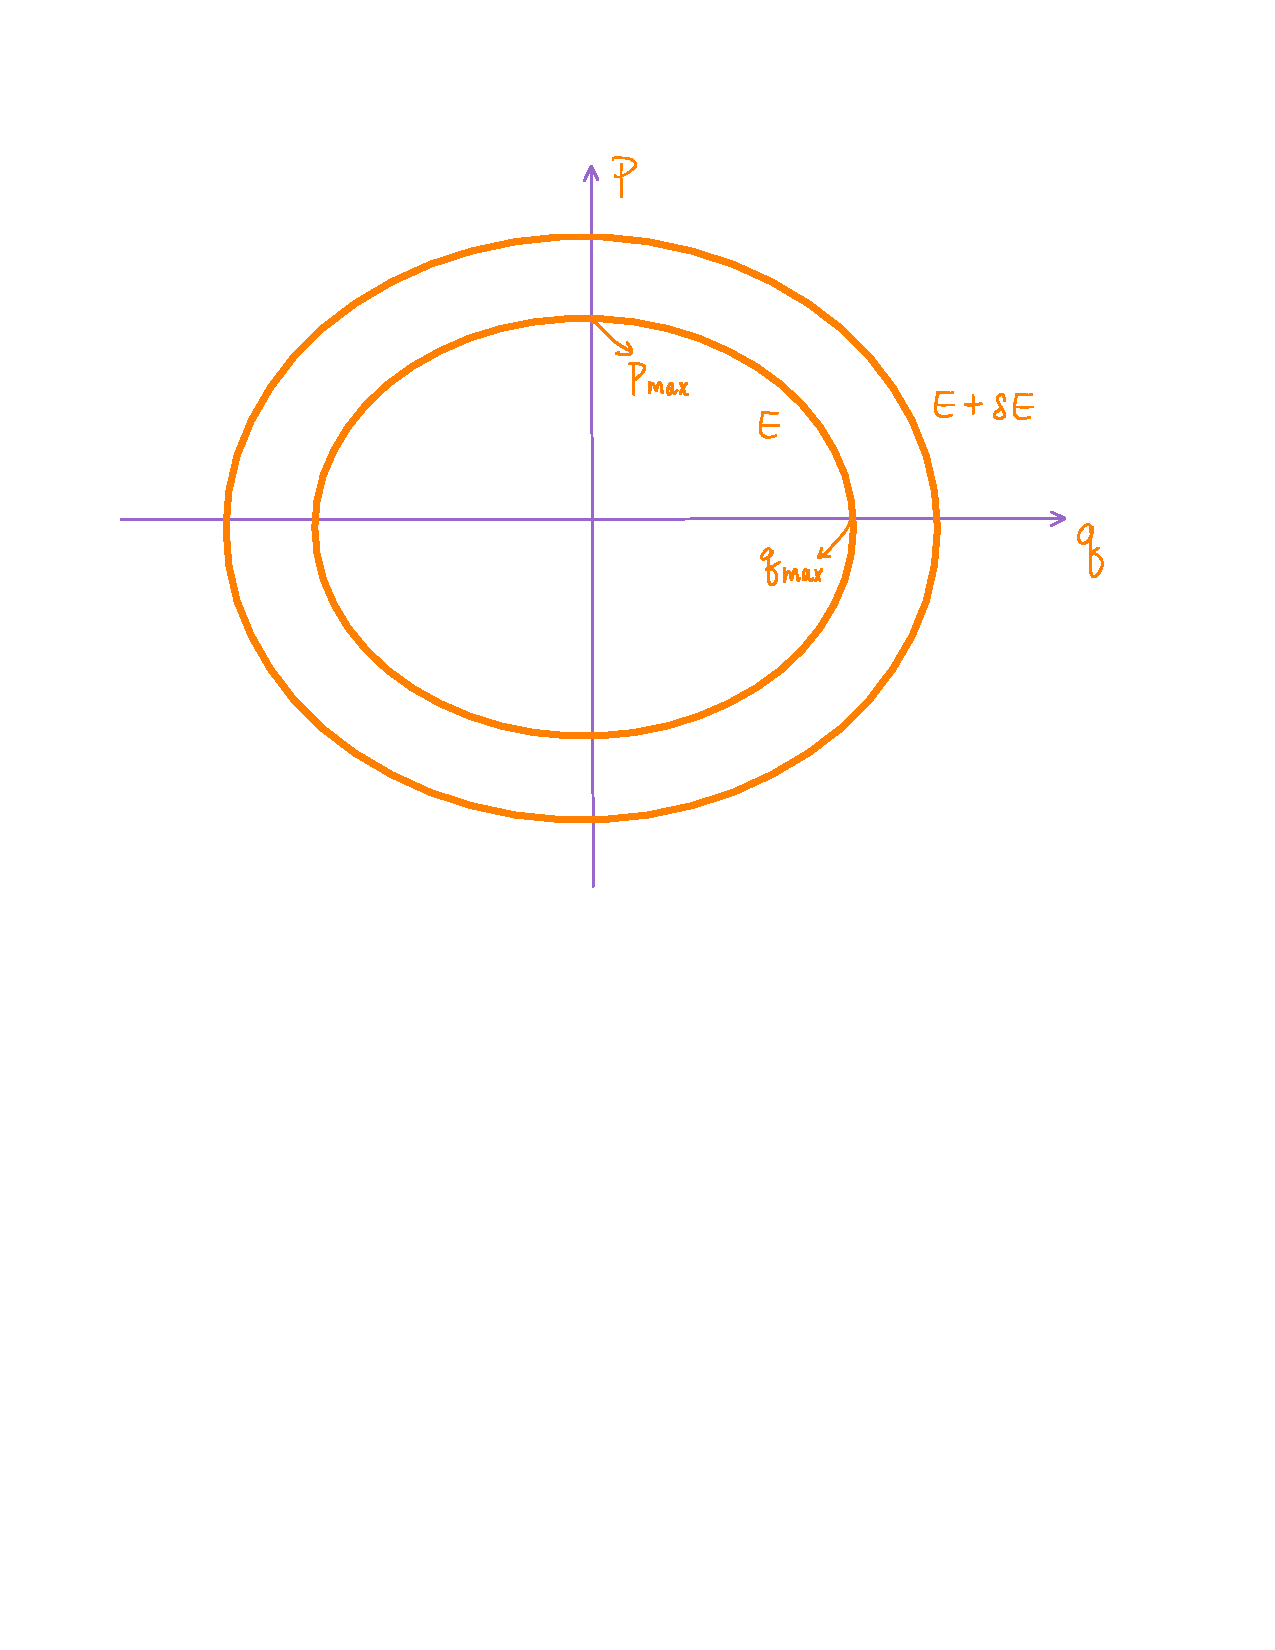
\includegraphics[scale=0.5]{pqPhaseSpace.pdf}
\end{center}
Let $\Phi(E)$ be the number of microstates with energy less than or equal to $E$. Let $\Omega(E)$ be the number of microstates with energy with energy between $E$ and $E+\delta E$. Here we get the following:
$$\Phi(E) = \frac{\pi p_{max} \cdot q_{max}}{h_0} = \frac{\pi (2mE)}{h_0(m\omega)} = \frac{E}{\frac{h_0}{2\pi} \omega}$$
For $\delta E << E$, we get the following:
$$\Omega(E) = \Phi(E+\delta E) - \Phi(E) = \frac{\partial \Phi}{\pd E}\delta E = \frac{\delta E}{\frac{h_0}{2\pi}\omega}$$

\hfill\break
Let $f$ be the degrees of freedom, $f$ momenta and $f$ coordinates. The dimension of phase space is them $2f$. Hence the volume of each cell in such phase space is given by: $$\delta q_1 \cdot \delta q_2 \cdot \cdots \cdot \delta q_f \cdot \delta p_1 \cdot \delta p_2\cdot \cdots \cdot \delta p_f = h_0^f$$


\example\\
For $1$-dimensional harmonic oscillation, with quantum theory, we can write:
$$E = \left(n+\frac{1}{2}\right) \hbar \omega$$
with $n\in \N$ being the energy level. A microstate is completely specified by a given $n$. Spacing between energy levels is $\hbar \omega$. Assuming $\delta E > \hbar \omega$, the number of microstates between $E$ and $E+ \delta E$ is then given by the following: 
$$\Omega(E) = \frac{\delta E}{\hbar \omega}$$
Comparing with what we get above for classical description of $1$-dimensional harmonic oscillation, the classical and the quantum description agree for $h_0 \approx h$, with $h$ being the Plank's Constant. \\
\newpage


\example\\
We would like to find the number of accessible microstates for a monatomic ideal gas of $N$ particles in a volume $V$. Note that there is no interaction between particles, so the total energy of such system is given by the following:
$$E = \sum_{i=1}^N \frac{||\vec{p}_i||^2}{2m}$$ which is the sum of the kinetic energy of all particle. Hence we get a constraint:
$$\sum_{i=1}^N (p_{ix}^2 + p_{iy}^2 + p_{iz}^2) = 2mE$$
For $3$-dimensional, suppose there are $N$ particles, each with $3$ degrees of freedom, so total of $3N$ degrees of freedom. The volume of each elementary region in the phase space is given by:
$$dq_1\cdot dq_2 \cdot \cdots \cdot dq_{3N}\cdot dp_1\cdot dp_2\cdot \cdots \cdot dp_{3N} = (h_0)^{3N}$$
Then we have: 
\begin{align*}
\Phi(E) &= \frac{1}{(h_0)^{3N}}\int dq_{1} \cdots dq_{3N} dp_1 \cdots dp_{3N}\\
&= \frac{1}{(h_0)^{3N}} \int dq_1 \cdot dq_2 \cdots \cdot dq_{3N} \int dp_1 \cdot dp_2 \cdots \cdot dp_{3N}
\end{align*}
Integrating over $dq_{1} \cdots dq_{3N}$ under the volume constraint $V$ gives $V^N$, and integrating over $ dp_1 \cdot dp_2 \cdots \cdot dp_{3N}$ under the constraint $\sum_{i=1}^N (p_{ix}^2 + p_{iy}^2 + p_{iz}^2) = 2mE$, which is a equation for a $3N$-dimensional sphere, gives $k(\sqrt{2mE})^{3N}$ for some constant $k$. Hence we can write:
$$\Phi(E) = \frac{k}{h_0} V^N E^{3N/2} \qquad \qquad \Omega(E) = \Phi(E + \delta E) - \Phi(E) \approx \frac{\partial \Phi(E)}{\partial E} \delta E = \frac{k}{h_0} V^N E^{\frac{3N}{2}-1} \delta E$$
The approximation for $\Omega(E)$ is obtained through Taylor Expansion of $\Phi$. \\

\example\\
For a particle trapped between two walls. Let $L$ be the distance between two walls, we get: $$E_n = \frac{\pi^2 \hbar^2}{2m} \left(\frac{n^2}{L^2}\right)$$ for $n \in \N$ being the quantum number. One can specify the microstate by giving $n$. \\
For a particle in a $3$-dimensional box, which dimension is given by $L_x\times L_y\times L_z$, 
$$E = \frac{\pi^2 \hbar^2}{2m}\left(\frac{n_x^2}{L_x^2} + \frac{n_y^2}{L_y^2}+ \frac{n_z^2}{L_z^2}\right) $$
where $n_x$, $n_y$ and $n_z$ are quantum numbers. One can specify the microstate by giving $n_x$, $n_y$, and $n_z$. \\

\hfill\break
\hfill\break
\newpage
A microcanonical ensemble describes an isolated system in equilibrium in which all microstates are equally probable. We use $\Omega(E)$ denote the number of microstates with energy between $E$ and $E+\delta E$, where $\delta E$ is greater than the amount of energy required to go between quantum levels in quantum theory. In the following we want to investigate how $\Omega(E)$ depends on $E$ for a system with high degrees of freedom. We will show in fact, by estimation, $\Omega(E) \propto E^f$ where $f$ is the number of degrees of freedom. In the following we denote $\Phi(E)$ as the number of microstates with energy less than or equal to $E$.\\


Consider a system of large number $(\geq 10^{23})$ degrees of freedom, and particles in such system are considered to be indistinguishable and non-interacting. Each degree of freedom, which could be considered as a particle moving in only one single direction, has its own energy levels. Let $\epsilon$ denote the energy of such particle, and $\Delta \epsilon$ denote the amount of energy required to go from one energy level to the consecutive one. For the entire system. Let $\Delta E$ denote the energy spacing between levels, with $\delta E > \Delta E$. Typically, we can write $\epsilon = \frac{E}{f}$. First note that, for $\delta E <<E$, we can write:
\begin{align*}
\Omega(E) = \Phi(E+\delta E) - \Phi(E) \approx \frac{\partial \Phi(E)}{\partial E}\delta E \tag{1}
\end{align*}
If two particles each has $m$ microstates with energy level less than $\epsilon$, then the total microstates in the system consisting of the two particles only, with energy level less than $E = 2\epsilon$, is $n^2$. With such argument, we can write the following:
$$\Phi(E) = \left(\Phi(\epsilon)\right)^f$$
Hence we can rewrite equation (1) as the following:
\begin{align*}
\Omega(E) \approx \frac{\partial \Phi(E)}{\partial E}\delta E =  (f)(\Phi(\epsilon))^{f-1}\left(\frac{\partial \Phi(\epsilon)}{\partial \epsilon}\frac{\partial \epsilon}{\partial E}\right) \delta E \tag{2}
\end{align*}
Notice that we also have:
$$\Phi(\epsilon) = \frac{\epsilon}{\Delta \epsilon} \quad \Rightarrow \quad \frac{\partial \Phi(\epsilon)}{\partial \epsilon} = \frac{1}{\Delta \epsilon}\qquad\qquad\qquad\qquad\qquad\qquad \epsilon = \frac{E}{f}\quad \Rightarrow \quad \frac{\partial \epsilon}{\partial E} = \frac{1}{f}$$
Hence equation (2) can be rewritten as the following:
$$\Omega(E)  = (f)(\Phi(\epsilon))^{f-1}\left( \frac{1}{\Delta \epsilon}\frac{1}{f}\right) \delta E = (\Phi(\epsilon))^{f-1} \frac{\delta E}{\Delta \epsilon}$$
One can show that $\Phi(\epsilon) \propto \epsilon^\alpha$ with $\alpha$ of order $1$, then we can write: 
$$\Phi(\epsilon) = \Phi(E/f) \propto E \qquad \Rightarrow \qquad \Omega(E) \propto E^{f-1} \frac{\delta E}{\Delta \epsilon}$$
Here we observe that we have: 
$$\ln(\Omega(E)) = (f-1)\ln (E) + \ln \left( \frac{\delta E}{\Delta \epsilon}\right) + constant$$
so for a good approximation, we have
$$\ln(\Omega(E)) \approx f\ln(E) + constant$$
or we have 
$$\Omega(E) \propto E^f$$
when $f$ is large enough. Here we see that $\Omega(E)$ is a rapidly varying function of $E$.

\newpage

Now we will introduce interactions between subsystems of an equilibrium system. \\There are two types of interaction: (1) the thermal interaction and (2) the mechanical interaction. \\

\example\\
Consider an isolated system, denoted as $A^0$, composed of two parts, $A$ and $A'$, which are themselves not isolated. The systems $A$ and $A'$ are connected by a thermally conducting movable wall. Here we can specify the macrostate of $A^0$, with $N,\ V,\ E,\ $ etc. for both $A$ and $A'$. \\
\begin{center}
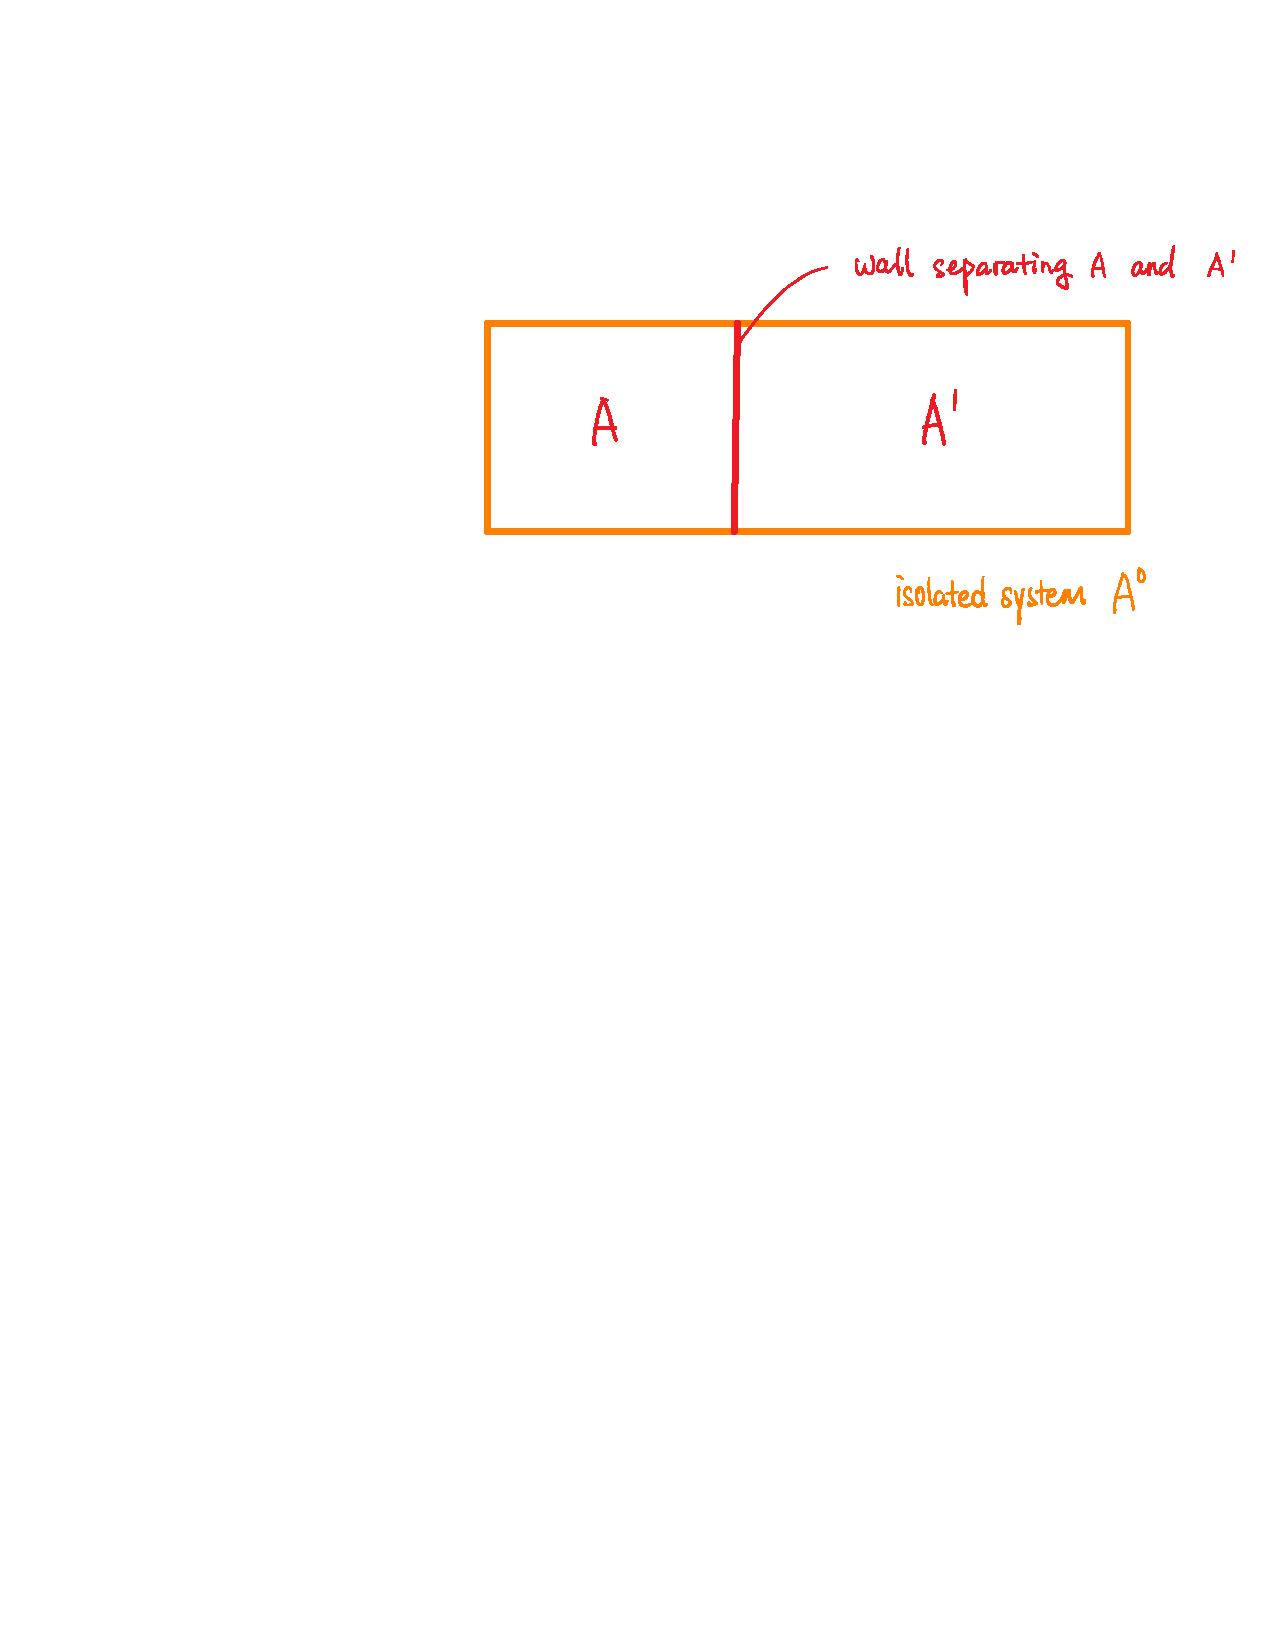
\includegraphics[scale=0.5]{interaction.pdf}
\end{center}

Note that energy is a function of external parameters. As we saw from the last example, particle in a $3$-dimensional box have $E\propto \frac{n_x^2}{L_x^2} +\frac{n_y^2}{L_y^2}+ \frac{n_z^2}{L_z^2}$, where $L_x, L_y, L_z$ are an external parameters. \\

In a macroscopic description, it is always useful to distinguish the two types of interaction, which are the thermal and mechanical interactions. For thermal interaction, external parameters of $A$ and $A'$ are fixed, but mean energies of $A$ and $A'$ will change. The mean energy transferred from one system to the other, say $A$ to $A'$, as a result of thermal interaction, and the energy transferred is called the heat. For mechanical interaction, external parameters of $A$ and $A'$, such as position of the wall separating $A$ and $A'$, will change, and one does work on the other. In this way, the mean energies of $A$ and $A'$ also change. \\

Also note that, when external parameters are kept fixed, then the energy for each probable microstate $E_r$ is fixed. If $\bar{E} = \sum_r p_r E_r$ changes, with $E_r$ being fixed, then we know that $p_r$ must have been changed.   \\

Microscopically, consider a single particle in a $1$-dimensional box.\\
First we consider a purely thermal interaction. 
\begin{center}
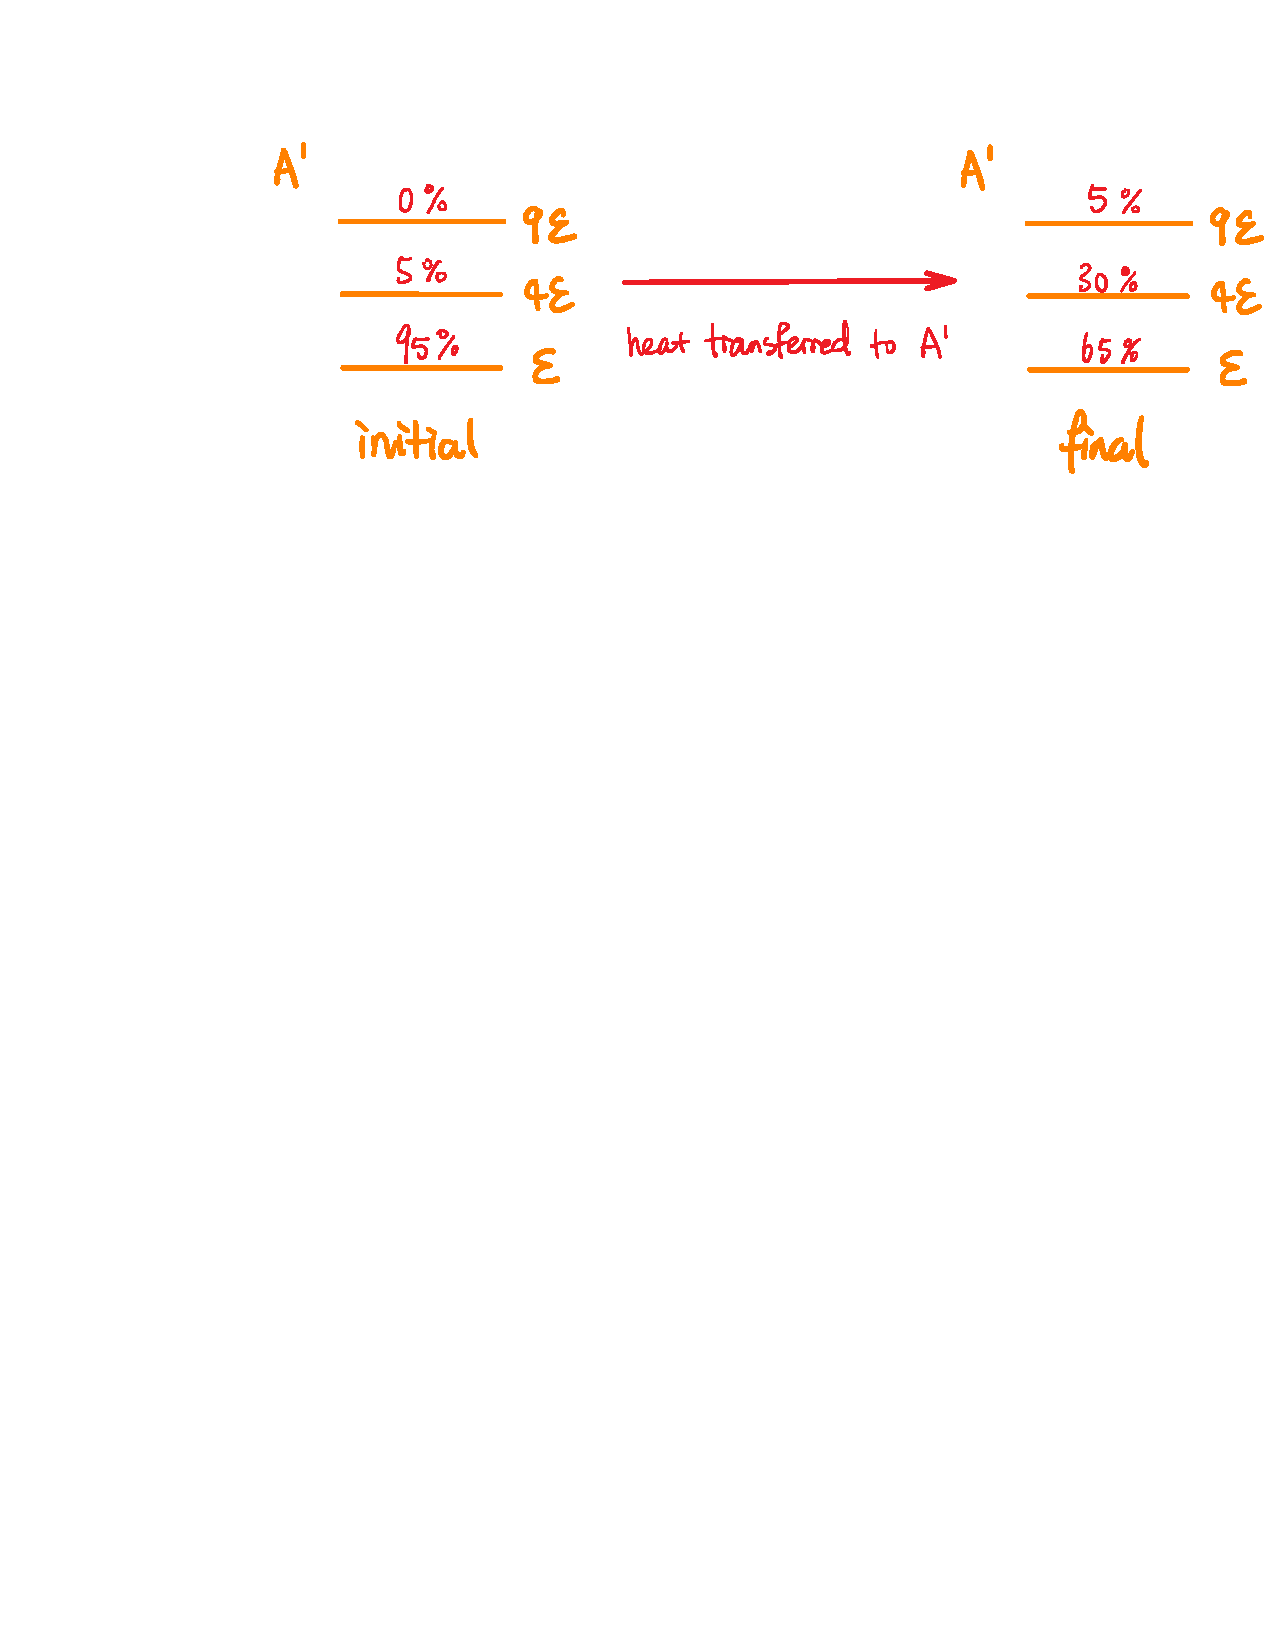
\includegraphics[scale=0.5]{thermalInteraction.pdf}
\end{center}
Here we can write:
$$\bar{E}_{intial} = 0.95 \epsilon + (0.05)(4\epsilon) = 1.15\epsilon$$
$$\bar{E}_{final} = 0.65 \epsilon + (0.3) (4\epsilon) + (0.05)9\epsilon = 2.3\epsilon$$
$$\text{Energy transferred: } Q = \Delta \bar{E} = 2.3\epsilon - 1.15\epsilon = 1.15\epsilon$$
Note that $E + E' = E^0$ is being fixed, where $E^0$ is the total energy of the system, $E,E'$ are energies for $A$ and $A'$, respectively. \\

Now consider a purely mechanical interaction. Here energy levels change. Say we compress $A'$ and make the wall between $A$ and $A'$ thermally insulating. As we do that, since the box of $A'$ is smaller, then the external parameters for $A'$ change. We compress $A'$ slowly such that $E^0$ is still fixed. 
\begin{center}
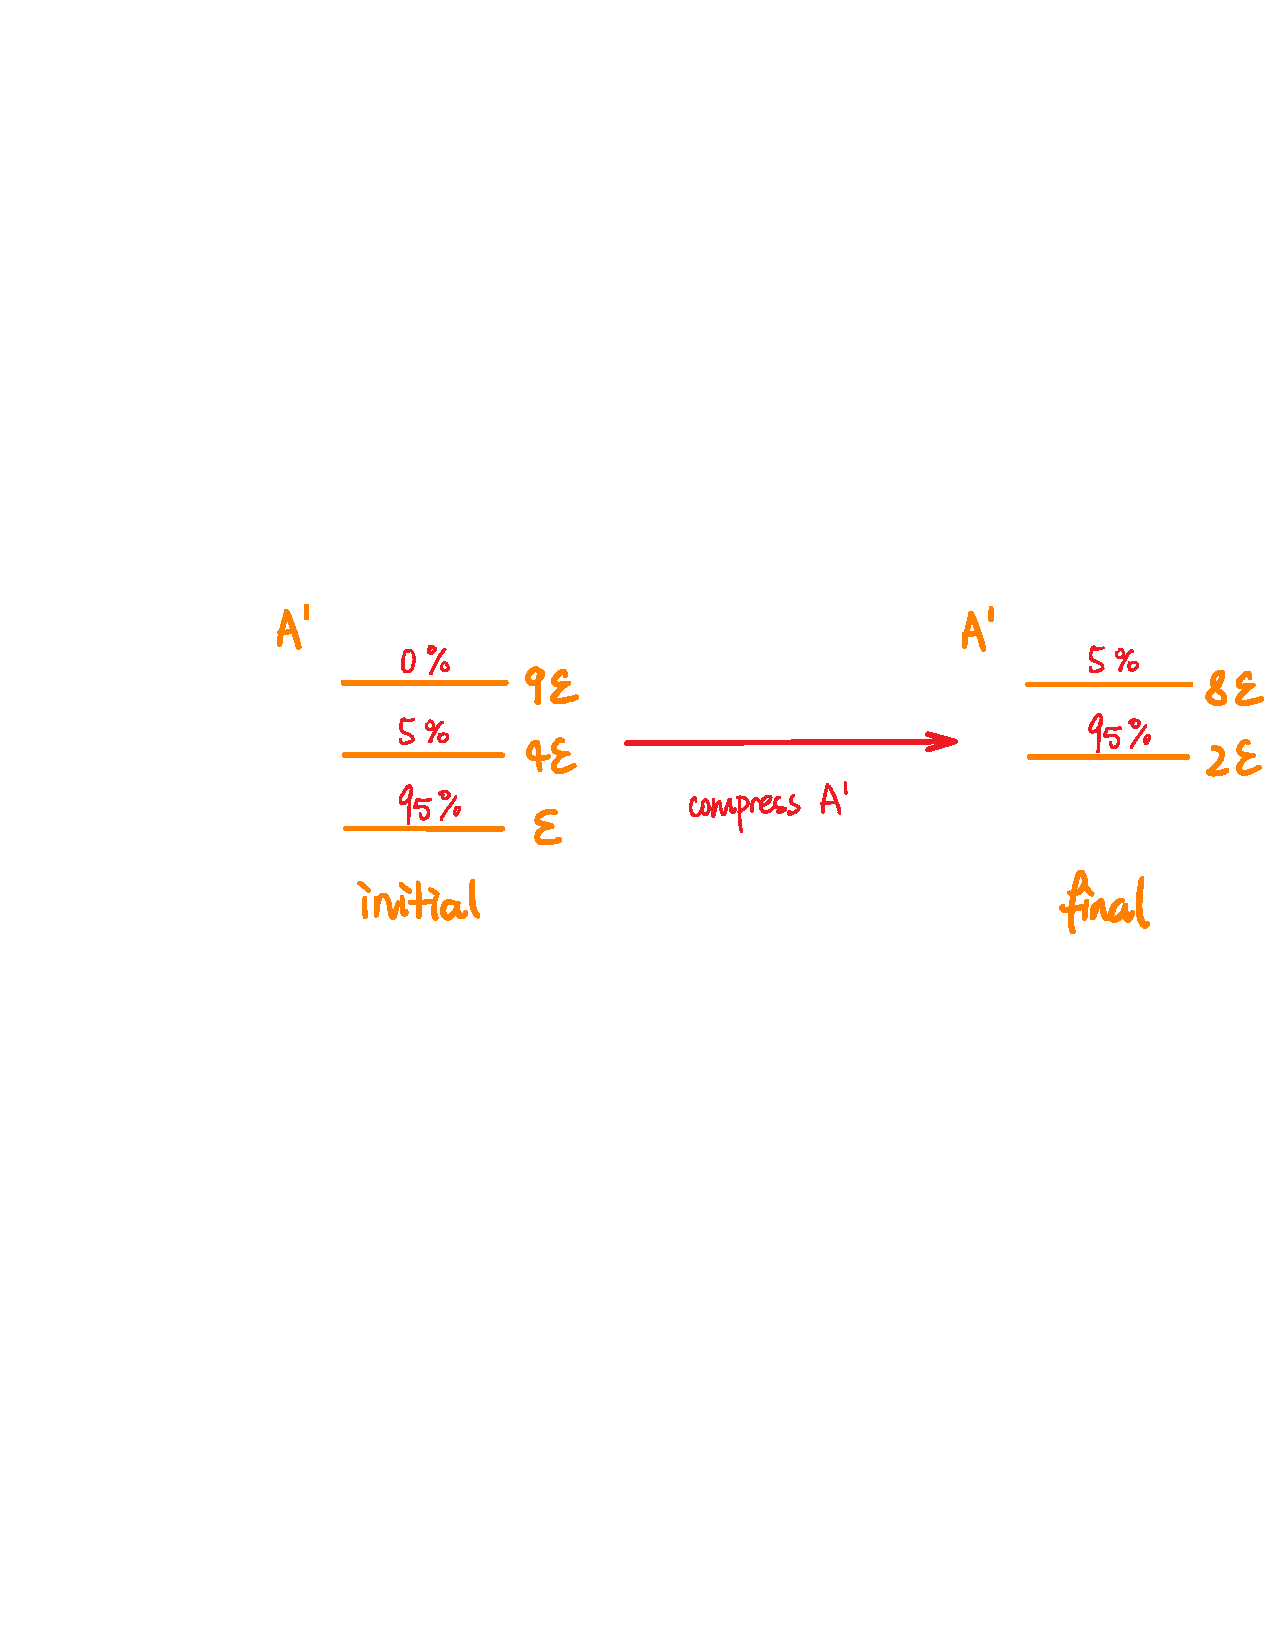
\includegraphics[scale=0.5]{mechanicalInteraction.pdf}
\end{center}
Now we can write:
$$\bar{E}_{initial} = 1.15\epsilon$$
$$\bar{E}_{final} = 2.3\epsilon$$
$$\text{Work done by }A' \text{ is given by }W = -\Delta \bar{E} = -1.15\epsilon$$


For a general interaction, both the external parameters change and the wall is thermally conducting, the division of energy transfer to heat and work is not so straightforward. Now consider a general interaction. That is, the wall of partition is thermally conducting and is movable. The average energy is given by:
$$\bar{E} = \sum p_r E_r$$
where both $p_r$ and $E_r$ might change. Now the division of energy transfer into heat and work is not well defined, in fact, they are process dependent. Energy is a function of external parameters, denoted as $E_r(x_1,x_2,\cdots, x_n)$, where $x_1,x_2,\cdots, x_n$ are external parameters, including volume, length, mechanic or electric field, and so on. Before interaction, we write $\bar{E} = \sum_r p_r E_r$. During interaction, $p_r$ could be changed to $p_r + \delta p_r$, and the external parameters would change, hence we have $E_r$ changes to $E_r + \delta E_r$, so the change in average energy is given by the following:
\begin{align*}
\overline{\Delta E} = \sum_r (p_r +\delta p_r)(E_r+\delta E_r) - \sum_r p_r E_r \tag{1}
\end{align*}
Now consider an infinitesimal change, which implies we could ignore the $\delta p_r \cdot \delta E_r$ terms, here we can rewrite equation (1):
\begin{align*}
\overline{\Delta E} = \sum_r \delta p_r E_r + \sum_r p_r \delta E_r \coloneqq \dbar Q -\dbar W
\end{align*}
here $\dbar W$ and $\dbar Q$ are not exact differentials. That is, we write:
$$\int_a^b \dbar W \neq W(b)-W(a)$$ 
Instead, $\int_a^b \dbar W$ is path dependent. Nevertheless, we will see that $\int_i^f \overline{ \Delta E} = E_f - E_i$, that is, $E$ depends only on endpoints, not the path, but both $\int_i^f \dbar Q$ and $\int_i^f \dbar W$ are both path dependent. \\


First, for $\sum_r p_r \delta E_r = -\dbar w$, as $E_r$ is a function of $x_1,x_2,\cdots, x_n$, we have:
\begin{align*}
\delta E_r = \sum_{\alpha=1}^n \frac{\partial E_r}{\partial x_{\alpha}}dx_{\alpha} \qquad \Rightarrow \qquad -\dbar W = \sum_r p_r \left(\sum_{\alpha} \frac{\partial E_r}{\partial x_{\alpha}}dx_{\alpha}\right) = \sum_{\alpha}\sum_r\left( p_r\frac{\partial E_r}{\partial x_{\alpha}}\right)dx_{\alpha}
\end{align*}
Hence we can define the generalized force as the following: 
$$\bar{X}_{\alpha} = -\sum_r p_r \frac{\partial E_r}{\partial x_{\alpha}} = -\frac{\partial \bar{E}}{\partial x_{\alpha}}$$
It follows that we can write: 
$$\dbar W = \sum_{\alpha} \bar{X}_{\alpha} dx_{\alpha}$$
$\bar{X}_{\alpha}$ is called the generalized force associated with the parameter $x_{\alpha}$. \\
Note that $\bar{X}_{\alpha}$ is a well defined macroscopic quantity.\\

Now $\dbar W = \sum_{\alpha} \bar{X}_{\alpha} dx_{\alpha}$ makses sense both microscopically and macroscopically. \\
To get a better sense of it, here we consider examples as the followings:\\

\example\\
Let $x_{\alpha}$ be volume. Then we have:
$$\bar{X}_{\alpha} = -\frac{\partial \bar{E}}{\partial V} = \bar{p} = \text{pressure}$$
Hence we can write $\dbar W = \bar{p}\, dV$. \\

Instead, if we have $x_{\alpha}$ being the length of a wire, then we have:
$$\bar{X}_{\alpha} = -\frac{\partial \bar{E}}{\partial l} = -\bar{T} = \text{tension}$$
Hence we can write $\dbar W = \bar{T}\, dV$.

\newpage
Now we will discuss the division of heat and work for finite process.\\

\begin{thm}[Finite Quasi-static Process]
In this process, the system stays close to equilibrium at all times.\\ For such a process, the work done is given by: 
$$W \coloneqq \int \dbar W = \int \sum_{\alpha} \bar{X}_{\alpha} dx_{\alpha}$$
Then we write:
$$Q \coloneqq \overline{\Delta E} + W$$
In general, both $Q$ and $W$ depend on the process, but $\overline{ \Delta E} = E_f - E_i$ depends only on the initial and final states, being path independent. In particular, $d\bar{E}$ is exact differential.
\end{thm}

Adiabatic process in one for which $\dbar Q = 0$, and in Quasi-static, we would write $Q= 0 $. \\

\example\\
If the only external parameter is $V$, the generalized force is then $p$. Any point on the $pV$-diagram specifies an equilibrium macrostate. Work done during a Quasi-static process is area under the curve, which depends on the process. \\

\example\\
We know that $\int_i^f dE = \int_i^f \dbar Q - \int_i^f \dbar W$, here we can write:
$$E_f - E_i = Q_{i\to f} - W_{i\to f}$$
For an Finite Quasi-static adiabatic process, we then have:
\begin{align*}
E_f - E_i = -W_{i \to f} = -\int p\, dV
\end{align*}

\hfill\break
More generally, $Q_{i\to f} = E_f - E_i + W_{i \to f}$. Here $E_f - E_i$ is measured mechanically in adiabatic process, and $W_{i \to f}$ is measured in process of interest.\\


Now consider a isolated system of equilibrium $A^0$, divided into two subsystems $A$ and $A'$, each with energy $E$ and $E'$ respectively, with $E^0 = E+E'$ being the total energy of $A^0$. Here $E^0$ is fixed as $A^0$ is an isolated system. Since $E^0$ is fixed, we take $E$ to be the only independent variable, and $E' \coloneqq E^0 - E$. The energy here is a function of both external $x_1,x_2,\cdots, x_n$ and internal parameters $y_1,y_2,\cdots, y_n$. Originally $A$ and $A'$ were separated by some constraint, now we remove the constraint between them and allow them to interact, in terms of both heat transfer and work. After interaction, the number of states accessible to the system increases. The most likely values of the internal parameters $y_1,y_2,\cdots,y_n$ after interactions are those that maximize missing information, here we denote the missing information as $\Omega(y_1,y_2,\cdots, y_n)$.\\

Consider first a purely thermal interaction, let $\Omega^0$ be the number of microstates accessible to $A^0$. Let $\Omega(E)$ be the number of states accessible to $A$, and $\Omega'(E')$ be the number of states accessible to $A'$. With energy for $A$ between $E$ and $E+\delta E$.
Here we have:
$$\Omega^0(E^0) = \Omega(E) \cdot \Omega' (E')$$
Recall that $\Omega(E)$ is a rapidly increasing function of $E$ as $E$ increases, with $\Omega(E) \propto E^f$ with $f$ being the degrees of freedom. $\Omega'(E') = \Omega'(E^0-E)$ is a rapidly  decreasing function of $E$ as $E $ increases. So the product will have a very sharp maximum. To maximize missing information, we want to maximize $\Omega^0(E^0)$. 
\begin{align*}
 \ln \Omega^0(E^0) = \ln \Omega(E) + \ln \Omega' (E')
\end{align*}
we have:
$$\frac{\partial \Omega^0(E^0)}{\partial E} = 0 \text{ at the maximum}$$
hence it follows that:
\begin{align*}
\frac{\partial }{\partial E}\ln \Omega(E) + \frac{\partial }{\partial E}\ln \Omega'(E') = 0 = \frac{\partial}{\partial E} \ln \Omega(E) - \frac{\partial }{\partial E'}\ln \Omega'(E') \tag{T}
\end{align*}
Here maximizing the missing information requires to find the condition that maximize $\Omega^0$. In such case, the two subsystems, with the new $E$ and $E'$ that maximize $\Omega^0$, is in equilibrium. Then here we have a way to define the temperature of the system $A^0$.
Rearranging equation (T) we get:
\begin{align*}
\frac{\partial }{\partial E}\ln \Omega(E) = \frac{\partial }{\partial E'}\ln \Omega'(E')
\end{align*}

Now we define:
\begin{align*}
\beta(E) \coloneqq \frac{\partial}{\partial E}\ln (\Omega(E))\qquad\qquad\qquad\beta'(E') \coloneqq \frac{\partial}{\partial E'}\ln (\Omega'(E'))
\end{align*}
At equilibrium where $E = \widetilde{E}$, we get the following:
\begin{align*}
\beta(\widetilde{E}) = p'(E_0-\widetilde{E})
\end{align*}
this property defines the temperature of the system:
$$T \coloneqq \frac{1}{k\beta}$$
with some convenient constant $k$. Now we can defined missing information as $$S \coloneqq k\ln(\Omega)$$ 
so $\beta = \frac{1}{k}\frac{\partial S}{\partial E}$, or we can write $\frac{1}{T} = \frac{\partial S}{\partial E}$. \\


In equilibrium thermodynamics, temperature is defined by $T^{-1} =\frac{\partial S}{\partial E}$, where $S$ is called the entropy. This allows us to define $S =k\ln(\Omega)$ being the entropy of the system. \\

Now we will investigate some properties of the given definitions. \\
Expand $\ln(\Omega(E))$ around $E = \widetilde{E}$, we can write the following:
\begin{align*}
\ln(\Omega(E)) &= \ln(\Omega(\widetilde{E})) + \left.\frac{\partial}{\partial E}\ln(\Omega(E))\right|_{E=\widetilde{E}} \Delta E + \left.\frac{1}{2}\frac{\partial^2}{\partial E^2}\ln(\Omega(E))\right|_{E=\widetilde{E}} (\Delta E)^2 + \cdots \\
&= \ln(\Omega(\widetilde{E})) + \beta(\widetilde{E}) \Delta E - \frac{1}{2}\lambda(\widetilde{E})(\Delta E)^2 + \cdots\\
\end{align*}
with $\lambda(\widetilde{E}') \coloneqq -\left.\frac{\partial^2}{\partial E^2}\ln(\Omega(E)) \right|_{E = \widetilde{E}}$. Let $\widetilde{E}'\coloneqq E^0 - \widetilde{E}$, similarly, we get the following:
\begin{align*}
\ln(\Omega'(E')) = \ln(\Omega'(\widetilde{E}')) - \beta'(\widetilde{E}') \Delta E - \frac{1}{2}\lambda'(\widetilde{E}') (\Delta E)^2
\end{align*}
Here we get:
\begin{align*}
\ln(\Omega^0(E)) = \ln(\Omega(\widetilde{E})\cdot \Omega'(\widetilde{E}')) - \frac{1}{2}(\lambda+\lambda') (\Delta E)^2
\end{align*}

Therefore, we get that: 
\begin{align*}
\Omega^0(E) = K e^{-1/2(\lambda+\lambda')(\Delta E)^2} \tag{D}
\end{align*}
with some constant $K$ because $\ln(\Omega(\widetilde{E})\cdot \Omega'(\widetilde{E}'))$ is a constant. Equation (D) gives us a Gaussian distribution. The dispersion of the Gaussian distribution is given by:
\begin{align*}
\frac{1}{\sqrt{\lambda+\lambda'}} \coloneqq \Delta^* E
\end{align*}
The distribution tells us that energy lies between $\widetilde{E}$ and $\widetilde{E}' + \Delta^* E$.\\ 
Recall that we estimated that $\Omega(E) \propto E^f$, hence we can write:
\begin{align*}
\beta(E) = \frac{\partial }{\partial E}\ln(\Omega(E)) \propto \frac{f}{E}\qquad\Rightarrow\qquad \frac{1}{\beta} \propto \frac{E}{f}
\end{align*}
Hence energy per degree of freedom is proportional to $kT$. Here we also have:
$$\lambda - \frac{\partial \beta}{\partial E} \propto -\left(-\frac{f}{E^2}\right) = \frac{f}{E^2}$$
The fractional width of the distribution is then given by the following:
\begin{align*}
\frac{\Delta^*E}{E}=\frac{1}{E\sqrt{\lambda}} \propto  \frac{1}{E\sqrt{\frac{f}{E^2}}} = \frac{1}{\sqrt{f}}
\end{align*}
which suggests that a system with large degrees of freedom would guarantee all definitions for entropy and temperature above well defined. 

\newpage
\textbf{Heat Reservoir}\\

Let $A^0$ be a system, $A$ and $A'$ be subsystems of $A^0$. Consider $A$ to be a large system, with many more degrees of freedom than $A'$, such that if heat flows from $A'$ to $A$, effective the temperature of $A$ does not change compared to the temperature change in $A'$. Let $\dbar Q$ denote the amount of heat flowing from $A'$ to $A$. All other parameters of $A'$ are kept fixed, that is, we assume $dE = \dbar Q$. Then we can write:
\begin{align*}
dS = \frac{\partial (k\ln(\Omega))}{\partial E'} \dbar Q = k \beta \dbar Q = \frac{k\dbar Q}{kT} = \frac{\dbar Q}{T}
\end{align*}
so when infinitesimal amount of heat flows into the system, entropy increases by $\frac{\dbar Q}{T}$. \\
Next consider finite heat transfer $Q$. We can write the following:
\begin{align*}
\Delta S = k\ln(\Omega(E+Q)) - k\ln(\Omega(E)) = k\frac{\partial \ln(\Omega)}{\partial E} Q + \frac{k}{2}  \frac{\partial^2 \ln(\Omega)}{\partial E^2}Q^2 + \cdots = k\beta Q + \frac{k}{2}\frac{\partial \beta}{\partial E} Q^2+\cdots  \tag{$\mathcal{S}$}
\end{align*}
but we found that: $$\beta \propto \frac{f}{E} \qquad \qquad \Rightarrow \qquad\qquad -\frac{\partial \beta}{\partial E} \propto \frac{f}{E^2}$$ 
so the second term of equation ($\mathcal{S}$) is of order $\left(\frac{Q}{E}\right)^2$. Therefore, the second term is small when $|\frac{Q}{E}|^2 <<1$, in which case system $A$ is called a heat reservoir, the second term vanishes, and we write the following:
\begin{align*}
 \Delta S = \frac{Q}{T}
\end{align*}


\begin{thm}[Zero-th Law of Thermodynamics]
The concept of temperature is useful in characterizing thermal equilibrium. There is no thermal interaction for systems with the same value of $\beta$. If systems $A$ and $C$ are in thermal equilibrium, then we must have $\beta_A = \beta_C$. If systems $C$ and $B$ are in thermal equilibrium, then we must have $\beta_A = \beta_B$, hence we must have $\beta_A = \beta_B$. That is, if two systems is in thermal equilibrium with a third system are in equilibrium with each other, then the third system is called a thermometer. 
\end{thm}
\newpage


Consider an isolated system in equilibrium $A^0$ with separated subsystems $A$ and $A'$, each with energy $E$ and $E'$ respectively, and volumes $V$ and $V'$ respectively. Just as we related $\frac{\partial }{\partial E}\ln (\Omega)$ to macroscopic $T$, we want to relate $\frac{\partial}{\partial X}\ln(\Omega)$ to generalized force $X = -\frac{\partial \bar{E}}{\partial x}$. Consider purely mechanical interaction. Energy is a function of external parameter $x$, when $x$ changes, energy goes from $E$ to $\frac{\partial E}{\partial x} \, dx$. Assuming that $\frac{\partial E}{\partial x}$ is same for all energy levels. Let $\Omega(E_1,x_1)$ denote the microstate accessible to energy $E_1$ with external parameter $x_1$. Since the interaction is purely mechanical, here we get:
\begin{align*}
\Omega\lr{E- \frac{\partial E}{\partial x}\, dx, x} = \Omega(E, x + dx)
\end{align*}  
Here we get the following by expanding the LHS through Taylor polynomial to leading order:
\begin{align*}
\Omega(E, x) - \frac{\partial \Omega}{\partial E} \frac{\partial E}{\partial x}\, dx = \Omega(E,x) + \frac{\partial\Omega}{\partial x}\, dx
\end{align*}
rearranging we get:
\begin{align*}
\frac{1}{\Omega}\frac{\partial \Omega}{\partial x} &= -\frac{1}{\Omega}\frac{\partial \Omega}{\partial E}\frac{\partial E}{\partial x}\\
\frac{\partial }{\partial x}\ln(\Omega) &= - \frac{\partial }{\partial E}\ln(\Omega) \cdot \frac{\partial E}{\partial x}\\
\frac{\partial}{\partial x}\ln(\Omega)&= \beta\left(-\frac{\partial E}{\partial x}\right)
\end{align*}
If $\frac{\partial E}{\partial x}$ is the same for all levels, we can replace $\frac{\partial E}{\partial x}$ by $\frac{\partial \bar{E}}{\partial x}$. 
Here we get:
\begin{align*}
\frac{\partial}{\partial x}\ln (\Omega) = \beta\left(-\frac{\partial\bar{E}}{\partial x}\right) = \beta X
\end{align*}
From here we get the Ideal gas law.\\

We have seen that for a non-interacting gas of $N$ particles in a volume $V$ with total energy $E$, we have the following:
$$\Omega = C V^N \chi (E)$$
where $C$ is a constant, and $\chi (E)$ is a function depending on the property of the gas. \\
For monoatomic gas, we have $\chi(E) = E^{3/2 N}$. Here we can write the following:
\begin{align*}
\ln (\Omega) = N\ln (V) + \ln (\chi(E)) + \text{constant}
\end{align*}
hence we have:
\begin{align*}
\frac{\partial}{\partial V}\ln(\Omega) = \frac{N}{V} = \beta \bar{p}
\end{align*}
where $\bar{p}$ is the pressure of the system, so we have $\bar{p}V = NkT$. \\

For monoatomic gas, we can write the following:
\begin{align*}
\ln(\Omega) = N\ln(V) + \frac{3}{2}N \ln(E) + \text{constant}
\end{align*}
hence we get:
\begin{align*}
\beta = \frac{\partial}{\partial E}\ln(\Omega) = \frac{3}{2}\frac{N}{E} = \frac{1}{kT} \qquad \Rightarrow\qquad E = \frac{3}{2}NkT
\end{align*}


Next consider what happens when both energy and external parameters change in infinitesimal interaction. Here we can write the following:
\begin{align*}
d\,\ln(\Omega)&= \frac{\partial \ln(\Omega)}{\partial E} d\bar{E} + \sum_{\alpha} \frac{\partial \ln(\Omega)}{\partial x_{\alpha}}dx_{\alpha}\\
&= \beta d\bar{E} + \sum_{\alpha} \beta X_{\alpha} dx_{\alpha}\\
&= \beta (dE + \sum_{\alpha} X_{\alpha}dx_{\alpha})
\end{align*}
For a Quasi-static proess, we have:
\begin{align*}
d \ln (\Omega)&= \beta(dE + \dbar W) = \beta \dbar Q \qquad \Rightarrow \qquad d(k\ln(\Omega)) = \frac{1}{T}\, \dbar Q = dS
\end{align*}


Concepts that can be described purely macroscopically includes equilibrium, Quasi-Static, adiabatic processes, thermometers, external parameters, generalized forces, work, and so on. Concepts that need some clarification includes temperature, internal energy. Concepts that need a lot of clarification includes entropy. The macroscopic ideas can be put together as the laws of thermodynamics.\\

The zero-th law of thermodynamics stated that two systems in thermal equilibrium with a third system are in thermal equilibrium with each other, which provides notion of temperature because we can define the third system as the thermometer. Here we note that $\beta$ itself is not clarified purely macroscopically.\\


\begin{thm}[First Law of Thermodynamics]
Every equilibrium macrostate of a system has a well defined internal energy $\bar{E}$ which is a constant for isolated system. For a thermally isolated system, we have the following holds:
\begin{align*}
E_f - E_i = -W_{i \to f}
\end{align*}
and in a general interaction, we have the following holds:
\begin{align*}
Q_{i\to f} = W_{i\to f} + E_f -E_i
\end{align*}
\end{thm}

\begin{thm}[Second Law of Thermodynamics]
Any equilibrium macrostate has a well defined entropy with the following properties:
\begin{enumerate}
\item For a thermally isolated system, we have $\Delta S |geq 0$ in any process.
\item In an infinitesimal Quasi-Static process, we get $\frac{\dbar Q}{T} = dS$
\end{enumerate}
\end{thm}

\begin{thm}[Third Law of Thermodynamics]
As temperature $T$ approaches $0$ from positive, we have $S$ approaches $0$. 
\end{thm}

These laws must be supplemented by statistical relation that we have:
\begin{align*}
S = k\ln(\Omega)
\end{align*}
where $\Omega$ is a function external and internal parameters. 

\newpage
\section{\color{red} Thermodynamics}
\subsection*{Math review}
There are two types of variables in Thermodynamics: 
\begin{enumerate}
\item The Extensive Variables are the variables which double when the system is doubled. That is, if we divide a system into two subsystems, those variables that are halved in the subsystem compared to the original system is called the extensive variables. Example includes volume, energy, entropy, and so on.
\item The Intensive Variables are the variables which stay the same when the system is doubled.  That is, if we divide a system into two subsystems, those variables that stay the same in the subsystem compared to the original system is called the extensive variables. Example includes temperature, pressure, and so on.
\end{enumerate}

In the theory of thermodynamics, we can calculate everything about a system if we know the fundamental relation: $S(E,V)$, that is, entropy $S$ as a function of energy $E$ and volume $V$. In such case, we can derive:
\begin{align*}
\frac{1}{T} = \left( \frac{\partial S}{\partial E}\right)_V \qquad\qquad\qquad \frac{p}{T} = \left( \frac{\partial S}{\partial V}\right)_E
\end{align*}
here the subscript denote the constant when taking a partial derivative. \\

The first derivatives of a fundamental relation are known as equations of state.\\

\example Ideal monatomic gas.\\
Here we have $S(E,V) = kN\ln(V) +\frac{3}{2}Nk \ln(E)+ \text{constant}$ which gives a fundamental relation. From here we see that:
\begin{align*}
\frac{1}{T} =  \left( \frac{\partial S}{\partial E}\right)_V = \frac{3}{2}\frac{Nk}{E} \qquad\qquad \Rightarrow\qquad\qquad E = \frac{3}{2}NkT \tag{1}
\end{align*}
\begin{align*}
\frac{p}{T} = \left( \frac{\partial S}{\partial V}\right)_E = \frac{Nk}{V} \qquad\qquad \Rightarrow\qquad\qquad pV = NkT \tag{2}
\end{align*}
here equation (1) and (2) are equations of state of the system, they give us full information of the system, namely the energy, volume, pressure, and so on. \\


\example Typical Problem in Thermodynamics.\\
Gas is expanded adiabatically, one might want to find how the temperature is changed during such process. Here $S$ is a constant. We can think of $T$ as a function of $S$ and $V$, then we can write:
\begin{align*}
dT = \left( \frac{\partial T}{\partial S} \right)_V \, dS + \left( \frac{dT}{dV}\right)_S \, dV = \left( \frac{\partial T}{\partial V}\right)_S dV
\end{align*}
By writing $dT$ as $dV = \left( \frac{\partial T}{\partial V}\right)_S dV$, we write it in terms of quantities which can be easily measured. \\

\newpage
\textbf{Manipulation with partial derivatives:}\\
Let $z(x,y)$ be a function of $x$ and $y$. Then we can write the followings:
\begin{align*}
dz = \left( \frac{\partial z}{\partial x}\right)_y \, dx + \left( \frac{\partial z}{\partial y}\right)_y \, dy
\end{align*}
Now suppose we fix $y$, that is, let $y$ be a constant, then $dy = 0$, hence we have:
\begin{align*}
dz = \left( \frac{\partial z}{\partial x}\right)_y \, dx 
\end{align*}
Now suppose instead, we fix $z$, that is, let $z$ be a constant, then we can write:
\begin{align*}
 \left( \frac{\partial z}{\partial x}\right)_y \, dx + \left( \frac{\partial z}{\partial y}\right)_y \, dy = 0 \qquad \qquad \Rightarrow \qquad \left( \frac{\partial x}{\partial y}\right)_z = - \frac{\left(\frac{\partial z}{\partial y} \right)_x}{\left(\frac{\partial z}{\partial x}\right)_y}
\end{align*}

Suppose we have a function $f(x,y)$ and we want partial derivatives of $f$, under the constraint $z(x,y) = $constant. Note here $z(x,y)$ being constant gives us a relation $x(y)$, or $y(x)$. Then we can write the following:
\begin{align*}
\left( \frac{\partial f}{\partial x}\right)_z &= \frac{d}{dx}f(x,y(x)) = \left( \frac{\partial f}{\partial x}\right)_y + \left( \frac{\partial f}{\partial y}\right)_x \left( \frac{\partial y}{\partial x}\right)_z 
\end{align*}

\begin{align*}
\left( \frac{\partial f}{\partial y}\right)_z &= \frac{d}{dx}f(x(y),y) = \left( \frac{\partial f}{\partial x}\right)_y \left( \frac{\partial x}{\partial y}\right)_z + \left( \frac{\partial f}{\partial y}\right)_x 
\end{align*}

Now we get:
\begin{align*}
\frac{\left( \frac{\partial f}{\partial x}\right)_z}{\left(\frac{\partial f}{\partial y}\right)_z} = \left( \frac{\partial y}{\partial x}\right)_z = \frac{ \left( \frac{\partial f}{\partial x}\right)_y + \left( \frac{\partial f}{\partial y}\right)_x \left( \frac{\partial y}{\partial x}\right)_z }{\left( \frac{\partial f}{\partial x}\right)_y \left( \frac{\partial x}{\partial y}\right)_z + \left( \frac{\partial f}{\partial y}\right)_x }
\end{align*}


Now we can relate the properties of partial derivatives to the fundamental relations. We have said that $S(E,V)$ is a fundamental relation, but one might also write $E(S,V)$, that is, energy as a function of entropy and volume. Here we get the equations of state as the followings:
\begin{align*}
\left(\frac{\partial E}{\partial S} \right)_V = \frac{1}{\left(\frac{\pd S}{\pd E} \right)_V} = \frac{1}{T^{-1}}  = T
\end{align*}
\begin{align*}
\left(\frac{\pd E}{\pd V} \right)_V = - \frac{\left( \frac{\pd S}{\pd V}\right)_V}{\left( \frac{\pd S}{\pd E}\right)_V} = -\frac{p/T}{1/T} = -p 
\end{align*}
\begin{align*}
dE = \left(\frac{\pd E}{\pd S} \right)_V \, dS + \left( \frac{\pd E}{\pd V}\right)_S \, dV = T\, dS - P\, dV = \dbar Q - \dbar W
\end{align*}


\example\\
Suppose we can write: $$S = Nk\ln (V) + \frac{3}{2}N k \ln(E) + C$$
with $C$ being a constant, then we can write:
\begin{align*}
\frac{S}{k} = \ln(V^n) + \ln(E^{3/2 N}) + K
\end{align*}
with $K$ being a constant. Then we can write:
\begin{align*}
E = A\, e^{\frac{2S}{3Nk}}\, V^{-2/3}
\end{align*}
with $A$ being a constant. One can check that the equation of state are the same as before.\\

\newpage
We want to look for other fundamental relation where the independent variables are different. The Legendre transformation allows us to do that.\\

Consider a function $y(x)$. The slope of the function is given by:
\begin{align*}
\rho \coloneqq \frac{dy}{dx}
\end{align*}
We want to construct a function of $\rho$ which will reconstruct $y(x)$. We call such function $\psi (\rho)$. The choice that works is letting $\psi(\rho)$ be the $y$ intercept of tangent line which the slope is $\rho$. 

\begin{align*}
\rho = \frac{y - \psi}{x-0} \qquad \Rightarrow \qquad\rho x = y-\psi \qquad \Rightarrow \qquad \psi = y-\rho x 
\end{align*}
\begin{align*}
\rho  = \frac{dy}{dx} = \rho(x) \qquad \Rightarrow \qquad y(x) = y(x(\rho))
\end{align*}

\example
\begin{align*}
y = x^2 \qquad \Rightarrow \qquad \frac{dy}{dx} = \rho = 2x \qquad \Rightarrow \qquad x = \frac{\rho}{2} \qquad \Rightarrow \qquad y = \lr{\frac{\rho}{2}}^2 = \frac{\rho^2}{4}
\end{align*}
Hence we have:
\begin{align*}
\psi = y - \rho x = \frac{\rho^2}{4} - \rho\cdot \lr{\frac{\rho}{2}} = -\frac{\rho^2}{4}
\end{align*}
\hfill\break
\hfill\break
\hfill\break
For reverse Legendre Transform, we have given $\psi$, we can write the following:
\begin{align*}
d\psi = dy - d\rho x - \rho dx
\end{align*}
Since $dy = \rho dx$, then we have:
\begin{align*}
d\psi = -xd\rho \qquad\Rightarrow \qquad \frac{d\psi}{d\rho}= -x
\end{align*}
That is, we have:
\begin{align*}
y(x) =  \psi(\rho(x)) + \rho(x)\cdot x
\end{align*}


\example.\\
The transformation from Lagrangian to Hamiltonian formulation is also an example of a Legendre transformation. For Lagrangian formulation, we have $L(q,\dot{q})$, with $\beta = \frac{\partial L}{\partial \dot{q}}$, we get $-H(p,q) = L(q,\dot{q}) - p \dot{q}$, or $H = p\dot{q}-L$. \\

\newpage
\textbf{Application of Legendre Transform to the Thermodynamics}\\

Starting with $E(S,V)$, $T = \lr{\frac{\pd E}{\pd S}}_V$, and $p = - \lr{\frac{\pd E}{\pd V}}_S$. We want to find a new equivalent fundamental relation with $T$, $V$ as fundamental relation. Let $y=E$, $x=S$, $T = \frac{\pd E}{\pd S} = \frac{d y}{dx} = \rho$, let the Legendre transform be $F(T,V)$, we get: $$F(T,V) = E- TS$$ 
which gives the Helmholtz Free Energy. Note here we can write:
\begin{align*}
dF = dE - TdS - SdT = TdS - pdV - TdS - SdT = -pdV - SdT
\end{align*}
here we see explicitly that $F$ is a function of $T$ and $V$. The equation of state is then given by:
\begin{align*}
\left(\frac{\pd F}{\pd V} \right)_T = -P \qquad \qquad \qquad \lr{\frac{\pd F}{\pd T}}_V = -S
\end{align*}
With the fact that partial derivatives commute, we see that:
\begin{align*}
 -\lr{\frac{\pd S}{\pd V}}_T =\left(\frac{\pd}{\pd V} \left(\frac{\pd F}{\pd T} \right)_V\right)_T = \lr{\frac{\pd}{\pd T} \lr{\frac{\pd F}{\pd V}}_T}_V = -\lr{\frac{\pd P}{\pd T}}_V
\end{align*}
That is, we get:
\begin{align*}
\lr{\frac{\pd S}{\pd V}}_T = \lr{\frac{\pd P}{\pd T}}_V
\end{align*}

Now we wan tot find fundamental relation with $S$, $P$ as independent variables. Here we have $E(S,V)$, $P = -\lr{\frac{\pd E}{\pd V}}_S$, let $E = y$ and $V = x$, $P = - \frac{\pd E}{\pd V} = -\frac{dy}{dx} = -\rho$, with Legendre Transform, we get $H = E+pV$, here $H(S,p)$ is called enthalpy. Here we can write the following:
\begin{align*}
dH = dE + pdV + Vdp = TdS - pdV + pdV + Vdp
\end{align*}
Rearranging we get:
\begin{align*}
\lr{\frac{dH}{dS}}_P = T \qquad \qquad \qquad \lr{\frac{dH}{dP}}_S = V
\end{align*}
From commutation of partial dervatives, we get:
\begin{align*}
\lr{\frac{\pd T}{\pd p}}_S = \lr{\frac{\pd V}{\pd S}}_p
\end{align*}
which gives us a Maxwell relation. \\

Now we want to find a fundamental relation with $T$, $p$ as fundamental variables. Now we do both Legendre transforms together, let $G(T,p)$ be the resulting fundamental relation, we can write:
\begin{align*}
G(T,p) = E-TS+pV
\end{align*}
Here $G(T,p)$ is called the Gibbs Free Energy. Note that we can write:
\begin{align*}
dG = dE - TdS - SdT + pdV+Vdp = TdS-pdV-TdS-SdT+pdV+Vdp = -SdT + Vdp
\end{align*}
Hence we get:
\begin{align*}
\lr{\frac{\pd G}{\pd T}}_P = -S \qquad\qquad\qquad \lr{\frac{\pd G}{\pd p}}_T = V
\end{align*}
and by commutation of derivatives, we have:
\begin{align*}
-\lr{\frac{\pd S}{\pd P}}_T = \frac{\pd V}{\pd T}_P
\end{align*}

Also recall that we can write:
\begin{align*}
\lr{\frac{\pd E}{\pd S}}_V = T \qquad\qquad\qquad \lr{\frac{\pd E}{\pd V}}_S = -p
\end{align*}
from here, by the commutation of derivatives, we can write:
\begin{align*}
-\lr{\frac{\pd p}{\pd S}}_V = \lr{\frac{\pd T}{\pd V}}_S
\end{align*}

Here we get the fundamental relations:
\begin{align*}
\begin{cases}
E(S,V) \\
F(T,V) =E-TS\\
H(S,p) =E+pV\\
G(T,p) =E-TS+pV
\end{cases}
\end{align*}
and the Maxwell's relations:
\begin{align*}
\lr{\frac{\pd p}{\pd T}}_V = \lr{\frac{\pd S}{\pd V}}_T \qquad&\qquad \qquad \lr{\frac{\pd T}{pd p}}_S = \lr{\frac{\pd V}{\pd S}}_p \\
-\lr{\frac{\pd S}{\pd p}}_T = \lr{\frac{\pd V}{\pd T}}_p\qquad&\qquad\qquad
-\lr{\frac{\pd p}{\pd S}}_V = \lr{\frac{\pd T}{\pd V}}_S
\end{align*}


In the following we will investigate the fundamental relations.\\

The total energy needed to create a system out of nothing in a constant pressure environment is given by the Enthalpy $H = E+pV$. In other words, the Enthalpy of a thermodynamic system is defined as the sum of its internal energy and the product of its pressure and volume. Here we assume that pressure $p$ is constant.\\

The total energy needed to create a system, subtracted by the heat one can get for free from the environment of constant temperature, gives us the Helmholtz Free energy $F=E-TS$, which is also the energy that must be provided as work if one wants to create the system from nothing. Conversely, if one annihilates the system, $F$ is the energy that comes out as work, and the other goes as heat dumped into the environment. In other words, $F$ denotes the available energy, or the free energy, at constant temperature $T$ of the environment.\\

The Gibbs Free Energy is just the sum of the effects in Enthalpy and Helmholtz Free Energy.\\

The issue remained is which of the fundamental relations has the most meaningful derivative. This requires us to determine which variables can be held fixed and which can be measured when varied.\\

$S$ can be held fixed in adiabatic process, while is not quite easy to be measured when changed because $dS = \frac{dQ}{T}$ and $dQ$ is hard to be measured.\\

$T$ is easy to be held fixed because one can just keep the system in constant temperature by using a heat bath. The change in temperature can also be measured using a thermometer.\\

$V$ is not easy to kept fixed because containers might expand when heat is added or removed, while its change is easy to be measured.\\

$p$ is easy to be kept fixed because we can keep the system in mechanically equilibrium with the atmosphere. The change in pressure is also easy to be measured by using a barometer.\\

Here we conclude that $T$ and $p$ are the most convenient variables. Here we see that $G(T,p)$ is the fundamental relation with the most meaningful derivative. \\

Here we get the standard form for the derivatives of $G(T,p)$, with independent variables $T$ and $p$.
\begin{align*}
\lr{\frac{\pd G}{\pd T}}_p = -S\qquad\qquad\qquad\qquad\qquad \lr{\frac{\pd G}{\pd p}}_T = V
\end{align*}
the second partial derivatives are given by:
\begin{align*}
\lr{\frac{\pd^2 G}{\pd T^2}}_p = -\lr{\frac{\pd S}{\pd T}}_p \coloneqq \frac{c_p}{T}
\end{align*}
where $C_p$ is specific heat at constant pressure. \\
Note here we write $\dbar Q = T dS$, and $\lr{\frac{dQ}{dT}}_p \coloneqq c_p$
\begin{align*}
\lr{\frac{\pd^2 G}{\pd p^2}}_T = \lr{\frac{\pd V}{\pd p}}_T \coloneqq V\kappa
\end{align*}
where $\kappa$ is the isothermal compressibility.\\
\begin{align*}
\lr{\frac{\pd^2 G}{\pd p \pd T}} = \lr{\frac{\pd V}{\pd T}}_p \coloneqq V\alpha
\end{align*}
where $\alpha$ is the volume coefficient of expansion under constant pressure. There are all the derivatives that we need for any thermodynamic experiments. \\

\begin{thm}
Any partial derivative of the form $\lr{\frac{\partial x}{\partial y}}_z$, where the set $\{x,y,z\}$ are any subset of $\{S,T,p,V,E,F,G,H\}$, can be expressed in terms of the first and second partial derivatives of a fundamental relation. $G(T,P)$ is usually the referred one because it has the most meaningful derivative. 
\end{thm}
The proof of this theorem follows from the derivative crasher algorithm. \\

We first name the following steps:
\begin{align*}
\lr{\frac{\pd x}{\pd y}}_z = \frac{1}{\lr{\frac{\pd y}{\pd x}}_z} \qquad\qquad\qquad\text{bring the }y \text{ to the nemurator}
\end{align*}
\begin{align*}
\lr{\frac{\pd x}{\pd y}}_z = -\frac{\lr{\frac{\pd z}{\pd y}}_x}{\lr{\frac{\pd z}{\pd x}}_y} \qquad\qquad\qquad\text{bring the }z \text{ to the nemurator}
\end{align*}
\begin{align*}
\lr{\frac{\pd x}{\pd y}}_z = -\frac{\lr{\frac{\pd x}{\pd w}}_z}{\lr{\frac{\pd y}{\pd w}}_z} \qquad\qquad\qquad\text{introduce new variable }w
\end{align*}
\textbf{Step 1.} Being potentials $(E,F,G,H)$ to numerator and eliminate the potentials one by one, so that the only remaining terms are $(S,T,V,P)$\\
\textbf{Step 2.} Bring $S$ to the numerator. Depending on which of $T,V,P$ are fixed, do the following:
\begin{enumerate}[topsep=3pt,itemsep=-1ex,partopsep=1ex,parsep=1ex]
\item At fix $T$, use Maxwell's relation $\lr{\frac{\pd S}{\pd V}}_T = \lr{\frac{\pd p}{\pd T}}_V$, $\lr{\frac{\pd S}{\pd p}}_T = -\lr{\frac{\pd V}{\pd T}}_p$
\item At fixed $V$ or $P$, introduce $T$ and write as specific heat $\lr{\frac{\pd S}{\pd T}}_p = \frac{c_p}{T}$, $\lr{\frac{\pd S}{\pd T}}_V = \frac{c_V}{T}$
\end{enumerate}
\textbf{Step 3.} Bring $V$ to the numerator to get $\alpha$ or $\kappa$.\\ 
\textbf{Setp 4.} Eliminate $c_V$ in terms of $c_p$, $\alpha$, and $\kappa$ by using the relation where $\lr{\frac{\pd f}{\pd x}}_z = \lr{\frac{\pd f}{\pd x}}_y + \lr{\frac{\pd f}{\pd y}}_x\lr{\frac{\pd y}{\pd x}}_z$.

\begin{align*}
\frac{c_V}{T} \coloneqq \lr{\frac{\pd S}{\pd T}}_V = \lr{\frac{\pd S}{\pd T}}_p + \lr{\frac{\pd S}{\pd p}}_T \lr{\frac{\pd p}{\pd T}}_V
= \lr{\frac{\pd S}{\pd T}}_V -\lr{-\frac{\pd V}{\pd T}}_p \frac{\lr{\frac{\pd V}{\pd T}}_p}{\lr{\frac{\pd V}{\pd p}}_T} = \frac{c_p}{T} -V\alpha \left(\frac{V\alpha}{V\kappa} \right) 
\end{align*}
Rearranging we get:
\begin{align*}
c_V = c_p - VT \frac{\alpha^2}{\kappa} \qquad\qquad\qquad c_p = c_V + VT\frac{\alpha^2}{\kappa}
\end{align*}
here we observe that $c_p > c_V$ for most systems. 

\example\\
In a thermodynamic experiment, one fixes $S$ and change $p$. 
\begin{align*}
dT = \lr{\frac{\pd T}{\pd p}}_S \, dp + \lr{\frac{\pd T}{\pd S}}_p \, dS &= \lr{\frac{\pd T}{\pd p}}_S \, dp
&= -\frac{\lr{\frac{\pd S}{\pd P}}_T}{\lr{\frac{\pd S}{\pd T}}_p}\, dp =  -\frac{-\lr{\frac{\pd V}{\pd T}}_p}{\lr{\frac{\pd S}{\pd T}}_p}\, dp = \frac{V\alpha}{c_p/T} = \frac{TV\alpha}{c_p} \, dp
\end{align*}





\end{document}
